% !TEX root = main.tex
\section{Experiments}
\subsection{Dataset}
Our dataset consists of 90 natural language instrauctions of which 60 are a sequence of simple move to instructions and 30 are high level natural language instructions. All these instructions are taken using a \href{http://52.25.65.189:9000/#/getFeedback}{crowd sourcing system} and the ground truth for the natural language instructions are also collected for evaluating the model. The instructions are taken for 16 different environments depicting scenes similar to living room, bedroom and kitchen. \\
The environments are constructed in OpenRAVE with context generating from 6 different human activities depicted by skeletals. The activities considered are walking, watching, interacting, reaching, sitting and working. \\
The instructions involve task description for themes in common house-hold enviromnent like cleaning the room, arranging the guest room and serving coffee and also some simple instructions like move to the bed and then to the table. The dataset contains considerable high level ambiguous instructions like distribute, arrange etc. with variety in verbs.\\
We filtered out 2 datapoints containing instructions which were very high level and uncertain even for  humans. Of the remaining 88 valid datapoints, 60 are used for training and 28 are used for testing purposes.  

% Please see supplementary for examples from our dataset.

\subsection{Set Up:}
	\subsubsection{Planit with Coactive Feedback:} 
		Planit is a crowd source platform that captures human interaction with the environment and learn their preferences over trajectories. Earlier version of planit was trained using expectation maximization using a database of 2500 trajectories over 112 different environments. In the current setting, we aim to to learn user preferences via coactive learning which requires a sub optimal feedback from the user which is more flexible to obtain and requires fewer number of training examples.

		Dataset consists of 16 different environments with 5 different activities occuring in them namely watching, walking, reaching, interacting, etc. User can view the environment in a simulator and can drag the robot to different positions in the environment. User provided the feedback in the form of a pair ($y,\bar{y}$) whereby $U(y) < U(\bar{y})$. This implies that the robot position $\bar{y}$ is more favourable for the user than the robot position $y$ in any trajectory in the environment. 

		Total 432 feedback was collected from the user across 10 different environment. For evaluation, we considered a set of 6 environments (not in the training set) from the dataset. The trained model was used to rank 112 trajectory sets each containing 7 trajectories to move between two randomly sampled points $A$ and $B$. Original version of planit (as reported in the planit paper (expert system) was assumed as the ground truth for evaluating the trajectories. The nDCG (normalized discounted cumulative gain) of \textbf{0.89} for the above model was observed. This is reasonable since in the earlier version the feedback was expert (labelling segments of 2500 different trajectories) and in the given system we have 400 instances of much weaker feedback.\ref{fig:planitResult} 


		% User was shown trajectories for going from one point to another and the user can stop trajectories and update specific waypoints of the trajectory by dragging the waypoint to a better point. 
		% 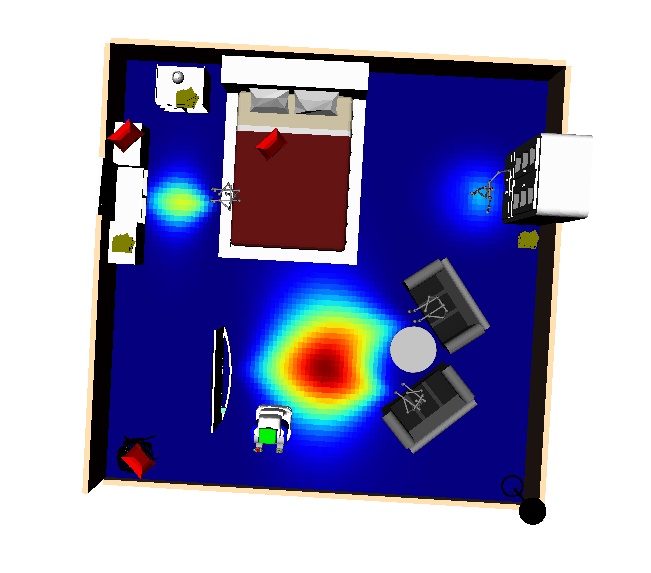
\includegraphics[scale=0.5]{planitResult}
		\begin{figure}[h]
		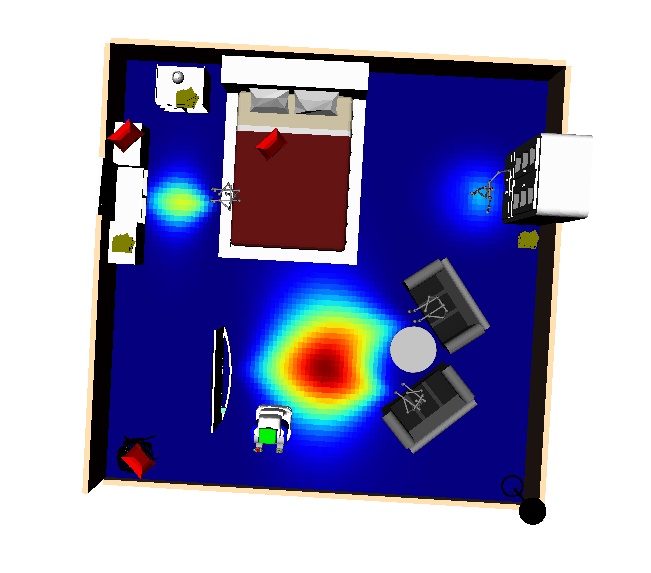
\includegraphics[width=8cm]{planitResult}
		\centering
		\caption{Cost function learnt via Coactive Feedback}
  		\label{fig:planitResult}
		\end{figure}


		\begin{figure}[h]
		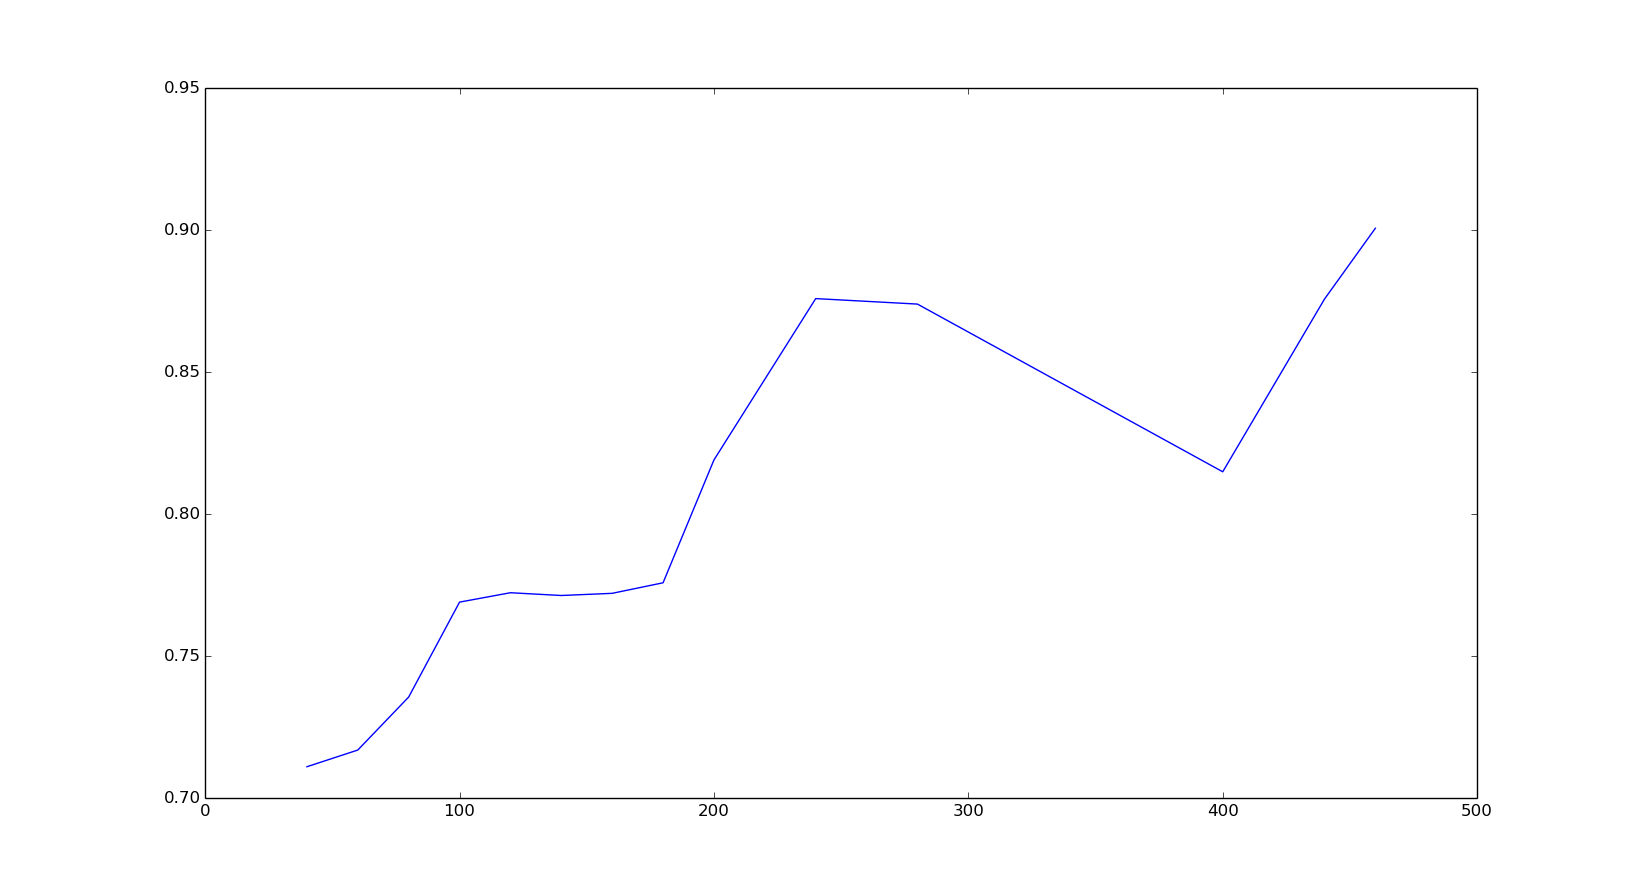
\includegraphics[width=9.5cm]{coactiveVSfeed}
		\centering
		\caption{Coactive Learning aginst number of feedbacks}
  		\label{fig:c1}
		\end{figure}
	\subsubsection{TellMeDave with Coactive Feedback:} 
		here goes description of tellmedave with coactive feedback

	\subsubsection{Joint system Coactive Feedback:}
		here goes description of the joint system with coactive feedback


\subsection{Results} \todo{Dip: please take a detailed pass over this subsection}
We test our algorithm on two tasks, in the first task we evaluate the success of co-active feedback in tuning the robot system and in second task, we evaluate the results from different type of feedback.

\noindent\textit{Task 1: Improvement Due to Co-active feedback}
\textit{Conclusion:} The system is able to improve its accuracy by BLAH on a held-out test set, after a few iterations of co-active feebacks from non-expert users.

\begin{table}
\label{tbl:tsk1}
\caption{Table 1: System improves its end-to-end accuracy after receiving co-active feedback on the final robot behavior}
\centering
\begin{tabular}{|l|l|}
\hline
\textit{System} & \textit{Accuracy} \\
\hline
Sys & BLAH \\
Sys + CF & BLAH \\
Sys + MCF & BLAH \\
\hline
\end{tabular}
\end{table}

\noindent\textit{Task 2: Effects of Different Type of Feedback}
\textit{Conclusion:} Our system based on co-active feedback is able to achieve close performance with system using expert feedback. Further, our system vastly outperforms system based on boolean feedback.

\begin{table}
\label{tbl:tsk2}
\caption{Table 2: Co-active feedback achieves close to the performance with expert feedback}
\centering
\begin{tabular}{|l|l|}
\hline
\textit{System} & \textit{Accuracy} \\
\hline
Sys + boolean & BLAH\\
Sys + CF & BLAH \\
Sys + Expert & BLAH \\
\hline
\end{tabular}
\end{table}


\todo{Dip: we should also experiment with individually tuning the two system AND experiment with different number of feedback until an asymptote is attained}
